\documentclass{article}
\usepackage{hyperref}
\usepackage{listings}
\usepackage{color}
\usepackage{geometry}
\usepackage{graphicx}
\usepackage{amsmath}
\usepackage{caption}
\usepackage{subcaption}
\geometry{margin=1in}
\pdfminorversion=6

\newcommand\TODO[1]{\textcolor{red}{TODO: #1}}

\newcommand\header[2]{
    \begin{center}
        {\large
        UCSD CSE 272 Assignment #1: \\
        \vspace{0.3cm}
        \Large
        #2}
    \end{center}
}

\definecolor{dkgreen}{rgb}{0,0.6,0}
\definecolor{gray}{rgb}{0.5,0.5,0.5}
\definecolor{mauve}{rgb}{0.58,0,0.82}
\lstset{frame=tb,
        aboveskip=3mm,
        belowskip=3mm,
        showstringspaces=false,
        columns=flexible,
        basicstyle={\small\ttfamily},
        numbers=none,
        numberstyle=\tiny\color{gray},
        keywordstyle=\color{blue},
        commentstyle=\color{dkgreen},
        stringstyle=\color{mauve},
        breaklines=true,
        breakatwhitespace=true,
        tabsize=2
}


\begin{document}

\header{1}{Disney Principled BSDF}

\begin{figure}[h]
    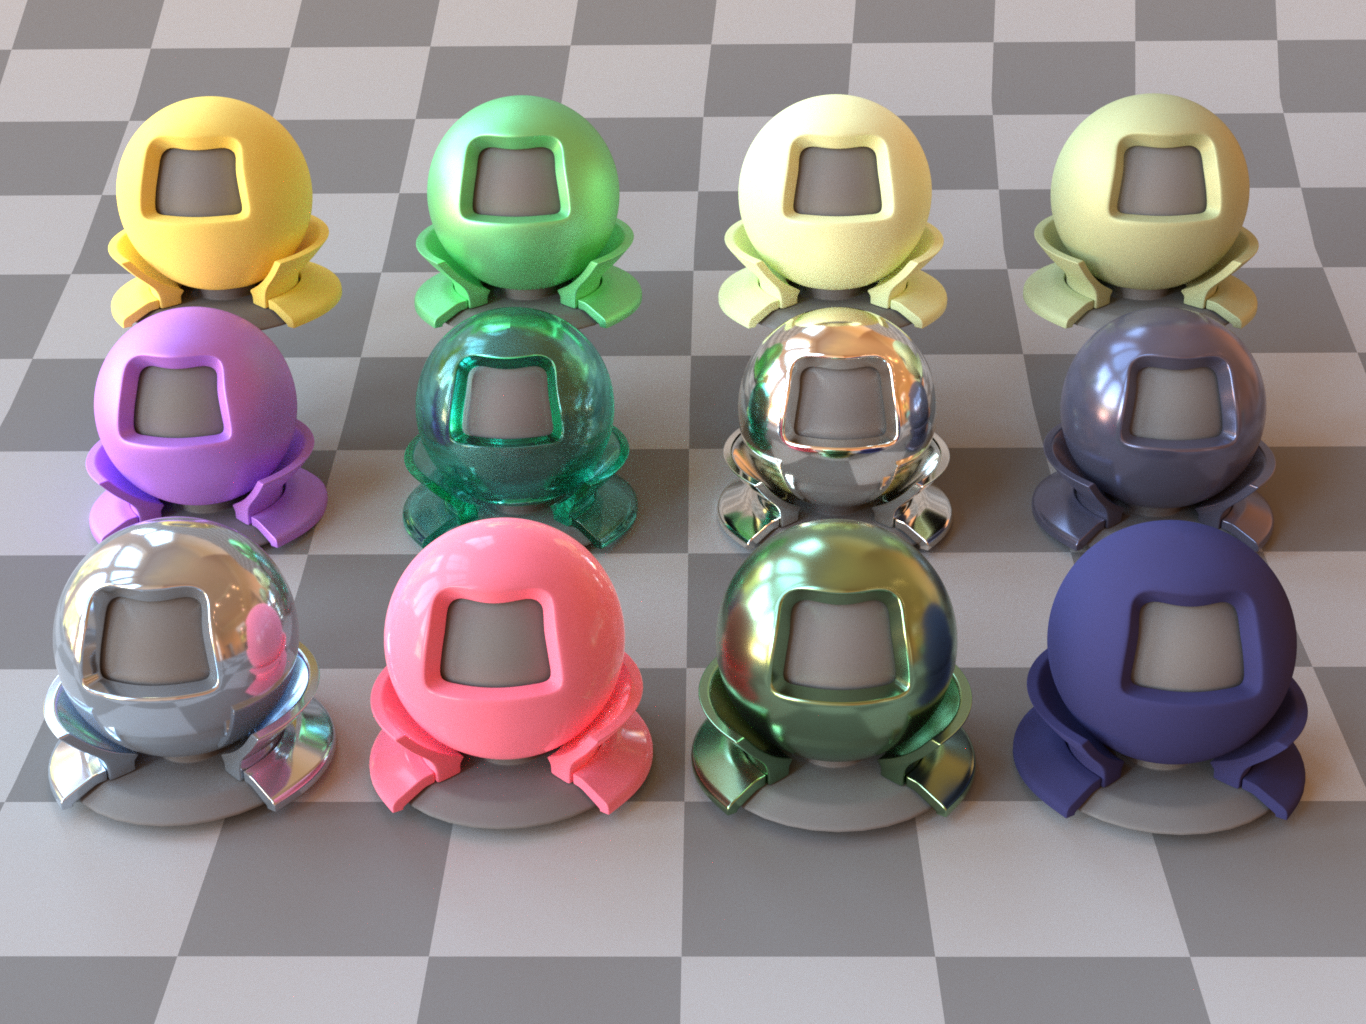
\includegraphics[width=\linewidth]{imgs/disney_bsdf.png}
    \caption{Disney principled BSDF~\cite{Burley:2012:PBS,Burley:2015:EDB} is a \emph{Uber shader} that can express a very wide range of materials.}
    \label{fig:gallery}
\end{figure}

In this homework, we will implement a Bidirectional Scattering Distribution Function, called the \emph{Disney principled BSDF} (Figure~\ref{fig:gallery}), in lajolla. Disney principled BSDF is an attempt to have a one-size-fits-all solution to cover most common materials using a single BSDF. It is \emph{principled} since it is (mostly) based on physical principles and observations from measured data~\cite{Matusik:2003:DRM}. However, physical correctness is not the utmost priority of the BSDF: it is a useful guideline for parameterizing the space of plausible materials for artistic expression. Ultimately, Disney BSDF is for making visual effects: as long as it makes graphics artists express what they want with the least effort, it achieves its goal. Disney BSDF has been extremely influential since its inception in 2012. Nowadays, many commercial and non-commercial rendering engines feature a similar material: \href{https://docs.blender.org/manual/en/latest/render/shader_nodes/shader/principled.html}{Blender's principled BSDF}, \href{https://autodesk.github.io/standard-surface/}{Autodesk's Standard Surface}, \href{https://docs.unrealengine.com/4.26/en-US/RenderingAndGraphics/Materials/PhysicallyBased/}{Unreal Engine 4's physically-based materials}, \href{https://substance3d.adobe.com/tutorials/courses/the-pbr-guide-part-1}{Substance's physically-based shaders}, and \href{https://appleseed.readthedocs.io/projects/appleseed-maya/en/master/shaders/material/as_standard_surface.html}{Appleseed standard surface}, are all heavily inspired, if not directly borrowed from the Disney BSDF.

We will implement the Disney BSDF with slight simplifications: first, we won't implement the full volumetric absorption/scattering model (we will implement something similar in the next homework!). Second, we remove a sheen transmissive lobe to make sampling easier. Finally, we do not implement the \emph{thin BSDF} model. When implementing the BSDF, feel free to reference code from the internet. However, be aware that due to the ambiguity in the Disney course note, all implementations I found are slightly different from each other, and some are flat out wrong.\footnote{Even the implementation in pbrt appears to be wrong. See \href{https://github.com/mmp/pbrt-v3/issues/313}{here}.} I found the following links to be useful: \href{https://github.com/wdas/brdf/blob/main/src/brdfs/disney.brdf}{the official implementation of the BRDF} (lacks the transmission component and no sampling procedures), \href{https://github.com/mmp/pbrt-v3/blob/master/src/materials/disney.cpp}{pbrt's implementation}, \href{https://schuttejoe.github.io/post/disneybsdf/}{Joe Schutte's walkthrough}, \href{https://github.com/knightcrawler25/GLSL-PathTracer/blob/master/src/shaders/common/disney.glsl}{a GLSL implementation}, and \href{https://github.com/dfelinto/blender/blob/master/intern/cycles/kernel/shaders/node_principled_bsdf.osl}{Blender's open shading language implementation}. The model we will implement is the closest to Blender's version. You should also read Burley's notes and presentations.\footnote{\url{https://blog.selfshadow.com/publications/s2012-shading-course/} and \url{https://blog.selfshadow.com/publications/s2015-shading-course/}}

A Disney BSDF is made of five components: a \textbf{diffuse} lobe that captures the base diffusive color of the surface, a \textbf{metallic} lobe that features major specular highlights, a \textbf{clearcoat} lobe that models the heavy tails of the specularity, a \textbf{sheen} lobe that addresses retroreflection, and a \textbf{glass} lobe that handles transmission. We will first implement each individual component; then we will combine all of them into a single material. 

\paragraph{Submission and grading.} Please upload a zip file to Canvas including your code, and a text file (readme.txt) answering the questions below. We will grade your code by comparing individual ray queries with our reference code for the BSDF evaluation, we will check if your sampling code is consistent with the PDF, and we will eyeball your rendering to make sure everything looks fine. For the questions, as long as you say something plausible, you will get full scores.

\paragraph{Notation and convention.} In the following, $\omega_{\text{in}}$ is the \emph{incoming} direction of the BSDF (usually represent the view direction), and $\omega_{\text{out}}$ is the \emph{outgoing} direction of the BSDF (usually represent the light direction), both pointing \emph{outwards} from the surface. $n$ is the shading normal, $n_g$ is the geometry normal, $h$ is the half-vector $h = \frac{\omega_{\text{in}} + \omega_{\text{out}}}{\|\omega_{\text{in}} + \omega_{\text{out}}\|}$. All of our BSDF include the cosine term $|n \cdot \omega_{\text{out}}|$. $\eta$ is the ratio of index of refraction of the medium below divided by the medium above the surface $\frac{\text{IOR}_{\text{internal}}}{\text{IOR}_{\text{external}}}$. All parameters of Disney BSDF are normalized within $[0, 1]$, except for the index of refraction whose acceptable range is $[1, 2]$.

\paragraph{Variant-based material systems.} As mentioned in homework 0, lajolla applies variant-based polymorphism instead of object-oriented polymorphism. The material \lstinline{struct}s in lajolla looks like the following:
\begin{lstlisting}[language=c++]
struct DisneyDiffuse {
    Texture<Spectrum> base_color;
    Texture<Real> roughness;
    Texture<Real> subsurface;
};
\end{lstlisting}
They are aggregated to a \lstinline{Material} type using variant.
\begin{lstlisting}[language=c++]
using Material = std::variant<Lambertian,
                              RoughPlastic,
                              RoughDielectric,
                              DisneyDiffuse,
                              DisneyMetal,
                              DisneyGlass,
                              DisneyClearcoat,
                              DisneySheen,
                              DisneyBSDF>;
\end{lstlisting}
Each material needs to implement the following operators:
\begin{lstlisting}[language=c++]
struct eval_op {
    Spectrum operator()(const Lambertian &bsdf) const;
    Spectrum operator()(const RoughPlastic &bsdf) const;
    Spectrum operator()(const RoughDielectric &bsdf) const;
    Spectrum operator()(const DisneyDiffuse &bsdf) const;
    // ...

    const Vector3 &dir_in;
    const Vector3 &dir_out;
    const PathVertex &vertex;
    const TexturePool &texture_pool;
    const TransportDirection &dir;
};

struct pdf_sample_bsdf_op {
    Real operator()(const Lambertian &bsdf) const;
    Real operator()(const RoughPlastic &bsdf) const;
    Real operator()(const RoughDielectric &bsdf) const;
    Real operator()(const DisneyDiffuse &bsdf) const;
    // ...

    const Vector3 &dir_in;
    const Vector3 &dir_out;
    const PathVertex &vertex;
    const TexturePool &texture_pool;
    const TransportDirection &dir;
};

struct sample_bsdf_op {
    std::optional<BSDFSampleRecord> operator()(const Lambertian &bsdf) const;
    std::optional<BSDFSampleRecord> operator()(const RoughPlastic &bsdf) const;
    std::optional<BSDFSampleRecord> operator()(const RoughDielectric &bsdf) const;
    std::optional<BSDFSampleRecord> operator()(const DisneyDiffuse &bsdf) const;
    // ...

    const Vector3 &dir_in;
    const PathVertex &vertex;
    const TexturePool &texture_pool;
    const Vector2 &rnd_param_uv;
    const Real &rnd_param_w;
    const TransportDirection &dir;
};
\end{lstlisting}

\section{Diffuse}
\begin{figure}
	\centering
	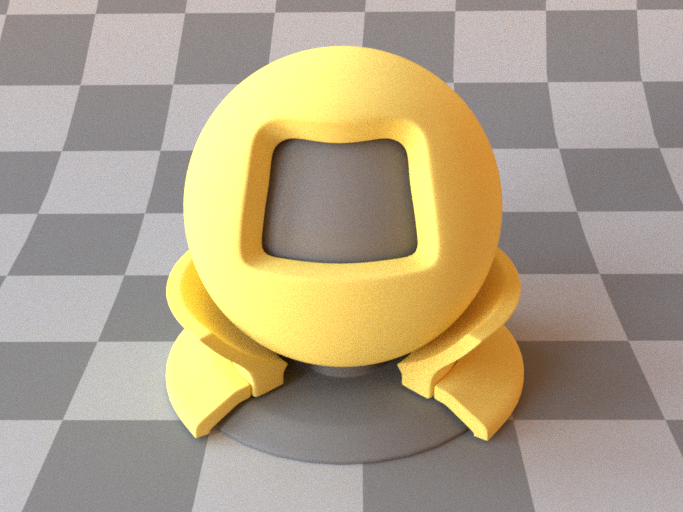
\includegraphics[width=0.5\linewidth]{imgs/disney_diffuse.png}
	\caption{Diffuse component of the Disney BSDF.}
\end{figure}

By looking at the MERL measured BRDF~\cite{Matusik:2003:DRM}, Burley found that at grazing retroreflection (when the half vector is roughly orthogonal to the normal), smooth materials (materials that are more specular) tend to have their reflectance dropped, and rough materials tend to have a peak at the grazing angle. The dropped reflectance can be predicted by Fresnel reflection: at grazing angles, (dielectric) Fresnel equation predicts low transmittance, and fewer lights are scattered inside the surfaces and thus less diffusion. Thus they design the following diffuse BRDF based on a modified version of the Schlick Fresnel approximation~\cite{Schlick:1994:IBM}:
\begin{equation}
	f_{\text{baseDiffuse}} = \frac{\text{baseColor}}{\pi}
	F_D(\omega_{\text{in}}) F_D(\omega_{\text{out}}) |n \cdot \omega_{\text{out}}|,
\end{equation}
where
\begin{equation}
\begin{aligned}
F_D(\omega) &= \left(1 + (F_{D90} - 1) (1 - |n \cdot \omega|)^5 \right) \\
F_{D90} &= \frac{1}{2} + 2 \cdot \text{roughness} \cdot |h \cdot \omega_{\text{out}}|^2.
\end{aligned}
\end{equation}

When $\text{roughness} = 0$ (smooth materials), at grazing view angle $|n \cdot \omega_{\text{in}}| \approx 0$, and at grazing lighting angle $|n \cdot \omega_{\text{out}}| \approx 0$, thus the BSDF attenuates the diffuse response by a factor of $\frac{1}{2}$ for each $F_D$ term (modelling the Fresnel reflection). At high roughness ($\text{roughness} \approx 1$), at retroreflection, $\omega_{\text{out}} \approx \omega_{\text{in}}$, thus $h \cdot \omega_{\text{out}} \approx 1$, and the BSDF reproduces the peak retroreflection observed in the MERL data by multiplying $2.5$ for each $F_D$ term.

In addition to the base diffuse model, the diffuse component of Disney BSDF also blends it with a subsurface scattering lobe for surfaces with strong multiple scattering inside like skin, milk, or marble. In the 2015 version of the Disney BSDF, they simulate \emph{real} subsurface scattering that requires volumetric path tracing to simulate the scattering, but this is too much work for the first homework. Instead, we follow the 2012 version and use a BRDF approximation of the subsurface scattering by modifying the Lommel-Seeliger law:
\begin{equation}
	f_{\text{subsurface}} = \frac{1.25 \text{baseColor}}{\pi} \left(
	F_{SS}(\omega_{\text{in}}) F_{SS}(\omega_{\text{out}}) \left(\frac{1}{|n \cdot \omega_{\text{in}}| + |n \cdot \omega_{\text{out}}|} - 0.5 \right) + 0.5 \right) |n \cdot \omega_{\text{out}}|,
\end{equation} 
where
\begin{equation}
\begin{aligned}
F_{SS}(\omega) &= \left(1 + (F_{SS90} - 1) (1 - |n \cdot \omega|)^5 \right) \\
F_{SS90} &= \text{roughness} \cdot |h \cdot \omega_{\text{out}}|^2.
\end{aligned}
\end{equation}

See \href{https://phys.libretexts.org/Bookshelves/Astronomy__Cosmology/Book%3A_Planetary_Photometry_(Tatum_and_Fairbairn)/03%3A_A_Brief_History_of_the_Lommel-Seeliger_Law/3.01%3A_A_Brief_History_of_the_Lommel-Seeliger_Law#:~:text=Description.,physical%20model%20of%20diffuse%20reflection.&text=Thus%2C%20of%20this%20diffuse%20scattered,emerging%20as%20diffuse%20reflected%20radiation.}{here} for a nice sketch of derivation of the Lommel-Seeliger law (brought to graphics by Hanrahan and Kruger~\cite{Hanrahan:1993:RLS}). The $\frac{1}{|n \cdot \omega_{\text{in}}| + |n \cdot \omega_{\text{out}}|}$ term models the volumetric absorption of the scattering media below the surface.

The final diffuse BRDF is:
\begin{equation}
	f_{\text{diffuse}} = (1 - \text{subsurface}) \cdot f_{\text{baseDiffuse}} + \text{subsurface} \cdot f_{\text{subsurface}},
	\label{eq:f_diffuse}
\end{equation}
where $\text{subsurface}$ is a parameter.

Note that the physical model here is a dielectric coating on top of a diffusive scattering media (similar to the \lstinline{roughplastic} material in lajolla/Mitsuba), but $f_{\text{diffuse}}$ does not model the specular reflection of the dielectric coating. We will include the specular reflection in the final assembly.

\paragraph{Task (10\%).} You will implement the \lstinline{DisneyDiffuse} BRDF (Equation~\ref{eq:f_diffuse})
\begin{lstlisting}[language=c++]
// in material.h
struct DisneyDiffuse {
    Texture<Spectrum> base_color;
    Texture<Real> roughness;
    Texture<Real> subsurface;
};
\end{lstlisting}

You need to implement the following three functions in \lstinline{materials/disney_diffuse.inl}:
\begin{lstlisting}[language=c++]
Spectrum eval_op::operator()(const DisneyDiffuse &bsdf) const;
Real pdf_sample_bsdf_op::operator()(const DisneyDiffuse &bsdf) const;
std::optional<BSDFSampleRecord> sample_bsdf_op::operator()(const DisneyDiffuse &bsdf) const;
\end{lstlisting}

For sampling, we will simply use a cosine hemisphere sampling. Look at \lstinline{materials/lambertian.inl} to see how it is done. Feel free to copy-paste the code and modify anything. Also notice how the Lambertian BRDF implementation handles the discrepancy between geometry normals and shading normals.

Try out the scene \lstinline{scenes/disney_bsdf_test/simple_sphere.xml} (you'll need to modify the scene file to use the \lstinline{DisneyDiffuse} material) and \lstinline{scenes/disney_bsdf_test/disney_diffuse.xml} to see how the material look like. Play with the parameters.

\paragraph{Questions (5\%).} Answer these questions in a text file:
\begin{enumerate}
	\item Compare the two BRDFs with a Lambertian BRDF: what differences do you see? Why?
	\item Compare the base diffuse BRDF ($f_{\text{baseDiffuse}}$) with the subsurface BRDF ($f_{\text{subsurface}}$) by playing with the subsurface parameter. What differences do you see? Why? In what lighting condition does the base diffuse BRDF differ the most from the subsurface BRDF? (Play with the light position in \lstinline{simple_sphere.xml} for your experimentation)
\end{enumerate}

\section{Metal}
\begin{figure}
	\centering
	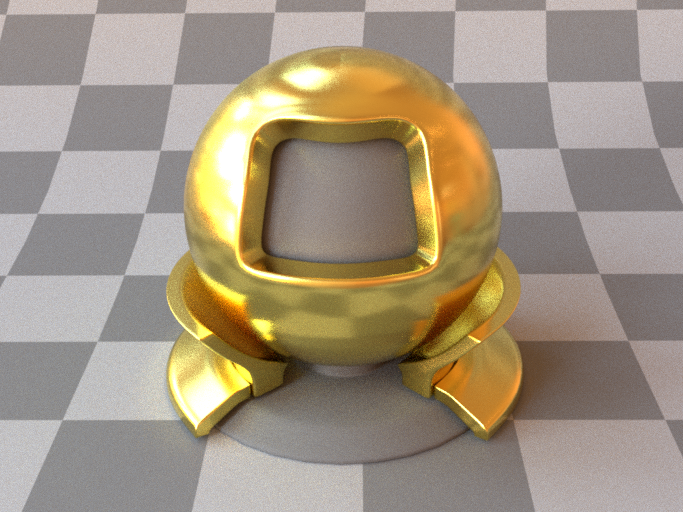
\includegraphics[width=0.5\linewidth]{imgs/disney_metal.png}
	\caption{Metal component of the Disney BSDF.}
\end{figure}

For specular reflection, Burley uses a standard Cook-Torrance microfacet BRDF~\cite{Cook:1982:RMC}:
\begin{equation}
f_{\text{metal}} = \frac{F_m D_m G_m}{4 |n \cdot \omega_{\text{in}}|},\footnote{The $|n \cdot \omega_{\text{out}}|$ term in the denominator cancels out with the cosine.}
\label{eq:f_metal}
\end{equation}
where $F_m$ is the Fresnel reflection, $D_m$ is the probability density of the distribution of a microfacet normal, and $G_m$ is the masking-shadowing term~\cite{Heitz:2014:UMF} that models the occlusion between microfacets.

For the Fresnel term $F_m$, Burley uses the Schlick approximation:
\begin{equation}
F_m = \text{baseColor} + (1 - \text{baseColor}) (1 - |h \cdot \omega_{\text{out}}|)^5.
\end{equation}
Note that the Fresnel term depends on the micronormal 
$h = \frac{\omega_{\text{in}} + \omega_{\text{out}}}{\left| \omega_{\text{in}} + \omega_{\text{out}} \right|}$ 
instead of the macro shading normal $n$. The reason why they use an approximation instead of the true Fresnel equation is not just for the performance. For metallic surfaces, or \emph{conductors}, Fresnel equation requires us to have the complex index of refraction of the conductor for each wavelength. This parameter is not only unintuitive, but nor is it physically accurate when we only consider the RGB spectrum.\footnote{See \href{http://renderwonk.com/publications/mam2019/}{``Fresnel Equations Considered Harmful''} by Naty Hoffman. \href{https://www.youtube.com/watch?v=kEcDbl7eS0w}{Here} is his presentation video.} 

For the normal distribution function $D_m$, Burley uses the anisotropic Trowbridge-Reitz distribution~\cite{Trowbridge:1975:AIR}, popularized by Walter et al.~\cite{Walter:2007:MMR} in graphics and it is known as \emph{GGX} (Ground Glass X):
\begin{equation}
D_m = \frac{1}{\pi \alpha_x \alpha_y \left(\frac{{h^l_x}^2}{\alpha_x^2} + \frac{{h^l_y}^2}{\alpha_y^2} + {h^l_z}^2\right)^2},
\end{equation}
where $h^l$ is the half-vector projected to the local shading frame. Physically, this models the distribution of the normals of an ellipsoid. Trowbridge-Reitz distribution was found to be fitting the MERL measured data excellently thanks to its heavy tails compared to a Gaussian or a cosine (some materials have even longer tails, and those will be modeled by the clearcoat component later). 

$\alpha_x, \alpha_y$ are parameters for modeling the smoothness of the material. If we directly use these parameters, we need very small $\alpha$ to represent highly specular materials. Burley found that the following mapping is more intuitive:
\begin{equation}
\begin{aligned}
\text{aspect} &= \sqrt{1 - 0.9 \text{anisotropic}} \\
\alpha_x &= max(\alpha_{\text{min}}, \text{roughness}^2 / \text{aspect}) \\
\alpha_y &= max(\alpha_{\text{min}}, \text{roughness}^2 \cdot \text{aspect})
\end{aligned},
\end{equation}
where $\text{anisotropic}$ and $\text{roughness}$ are the parameters.

Given a normal distribution function and a microfacet configuration, it is possible to derive the average occlusion factor $G_m$ given a viewing angle~\cite{Heitz:2014:UMF}. Burley uses the Smith model, which enables a closed-form solution under the assumption that all the microfacets are independently oriented:
\begin{equation}
\begin{aligned}
G_m &= G(\omega_{\text{in}}) G(\omega_{\text{out}}) \\
G(\omega) &= \frac{1}{1 + \Lambda(\omega)} \\
\Lambda(\omega) &= \frac{\sqrt{1 + \frac{\left(\omega_l.x \cdot \alpha_x\right)^2 + \left(\omega_l.y \cdot \alpha_y\right)^2}{\omega_l.z^2}} - 1}{2}
\end{aligned}.
\end{equation}

Combining all of these, and you will get a nice metallic BRDF.

\paragraph{Task (10\%).} You will implement the \lstinline{DisneyMetal} BRDF (Equation~\ref{eq:f_metal})
\begin{lstlisting}[language=c++]
// in material.h
struct DisneyMetal {
    Texture<Spectrum> base_color;
    Texture<Real> roughness;
    Texture<Real> anisotropic;
};
\end{lstlisting}

You need to implement the following three functions in \lstinline{materials/disney_metal.inl}:
\begin{lstlisting}[language=c++]
Spectrum eval_op::operator()(const DisneyMetal &bsdf) const;
Real pdf_sample_bsdf_op::operator()(const DisneyMetal &bsdf) const;
std::optional<BSDFSampleRecord> sample_bsdf_op::operator()(const DisneyMetal &bsdf) const;
\end{lstlisting}

For sampling, we will use the visible normal sampling developed by Heitz~\cite{Heitz:2018:SGD}, which importance samples $\frac{D_m G(\omega_{\text{in}})}{4 |n \cdot \omega_{\text{in}}|}$. See Heitz's presentation \href{https://jcgt.org/published/0007/04/01/slides.pdf}{slides} for a really nice illustration of the method. This sampling is also used in the \lstinline{roughplastic} material in lajolla, so you might want to look at it as well.

Try out the scene \lstinline{scenes/disney_bsdf_test/simple_sphere.xml} and the scene \lstinline{scenes/disney_bsdf_test/disney_metal.xml} to see how the material look like. Play with the parameters.

\paragraph{Questions (5\%).} Answer these question(s) in a text file:
\begin{enumerate}
	\item Compare \lstinline{DisneyMetal} with the \lstinline{roughplastic} material. What differences do you see?
	\item Change the roughness parameters. Apart from how specular the surface it, do you observe any other differences?
\end{enumerate}

\section{Clearcoat}
\begin{figure}
	\centering
	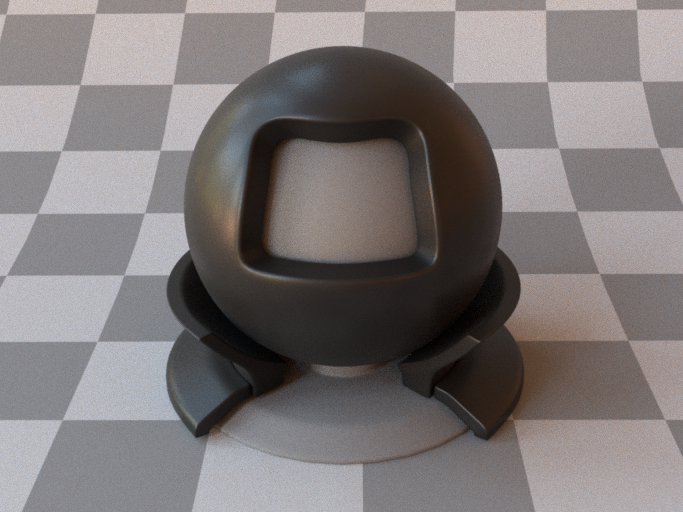
\includegraphics[width=0.5\linewidth]{imgs/disney_clearcoat.png}
	\caption{Clearcoat component of the Disney BSDF.}
\end{figure}

Burley found that the Trowbridge-Reitz distribution used by the metallic component above, while already having a wide tail comparing to most other normal distribution functions, is still not wide enough. Therefore they propose to have another achromatic specular component with a modified normal distribution function:
\begin{equation}
f_{\text{clearcoat}} = \frac{F_c D_c G_c}{4 |n \cdot \omega_{\text{in}}|},
\label{eq:f_clearcoat}
\end{equation}
where
\begin{equation}
\begin{aligned}
F_c &= R_0(\eta = 1.5) + (1 - R_0(\eta = 1.5)) \left(1 - |h \cdot \omega_{\text{out}}|\right)^5 \\
D_c &= \frac{\alpha_g^2}{\pi \log(\alpha_g^2) \left( 1 + (\alpha_g^2 - 1) \left(h^l_z\right)^2 \right)} \\
G_c &= G_{c}(\omega_{\text{in}}) G_{c}(\omega_{\text{out}}) \\
G_{c}(\omega_{\text{in}}) &= \frac{1}{1 + \Lambda_c(\omega)} \\
\Lambda_c(\omega) &= \frac{\sqrt{1 + \frac{\left(\omega_l.x \cdot 0.25\right)^2 + \left(\omega_l.y \cdot 0.25\right)^2}{\omega_l.z^2}} - 1}{2}
\end{aligned}.
\end{equation}
The Schlick Fresnel $F_c$ has a hard-coded index of refraction $\eta = 1.5$. The normal distribution function $D_c$ uses an isotropic roughness $\alpha = \alpha_g$. The masking-shadowing term $G_c$ uses a fixed roughness $0.25$. Note that this is an ad-hoc fit, and there is no clear geometric meaning of this microfacet BRDF.

The Schlick approximation maps the index of refraction $\eta$ to $R_0$ with the following equation:
\begin{equation}
R_0(\eta) = \frac{\left(\eta - 1\right)^2}{\left(\eta + 1\right)^2}
\end{equation}

The $\alpha_g$ parameter is mapped to a parameter $\text{clearcoatGloss}$ with the following equation:
\begin{equation}
\alpha_g = (1 - \text{clearcoatGloss}) \cdot 0.1 + \text{clearcoatGloss} \cdot 0.001.
\end{equation}
The higher the $\text{clearcoatGloss}$, the lower the $\alpha_g$.

\paragraph{Task (10\%).} You will implement the \lstinline{DisneyClearcoat} BRDF (Equation~\ref{eq:f_clearcoat})
\begin{lstlisting}[language=c++]
// in material.h
struct DisneyClearcoat {
    Texture<Real> clearcoat_gloss;
};
\end{lstlisting}

You need to implement the following three functions in \lstinline{materials/disney_clearcoat.inl}:
\begin{lstlisting}[language=c++]
Spectrum eval_op::operator()(const DisneyClearcoat &bsdf) const;
Real pdf_sample_bsdf_op::operator()(const DisneyClearcoat &bsdf) const;
std::optional<BSDFSampleRecord> sample_bsdf_op::operator()(const DisneyClearcoat &bsdf) const;
\end{lstlisting}

For sampling, there is no known visible normal sampling for this BRDF (since it does not correspond to a meaningful physical configuration). We will importance sample $\frac{D_c |n \cdot h|}{4 |h \cdot \omega_{\text{out}}|}$ by choosing a micro normal proportional to $D_c$ then reflect the incoming direction. To sample a normal $h^{l}$ in the local shading frame using a 2D random number $(u_0, u_1)$:
\begin{equation}
\begin{aligned}
\cos(h_{\text{elevation}}) &= \sqrt{\frac{1 - \left(\alpha^2\right)^{1 - u_0}}{1 - \alpha^2}} \\
h_{\text{azimuth}} &= 2 \pi u_1 \\
h^l_x &= \sin(h_{\text{elevation}}) \cos(h_{\text{azimuth}}) \\
h^l_y &= \sin(h_{\text{elevation}}) \sin(h_{\text{azimuth}}) \\
h^l_z &= \cos(h_{\text{elevation}})
\end{aligned}.
\end{equation}

Try out the scene \lstinline{scenes/disney_bsdf_test/simple_sphere.xml} and the scene \lstinline{scenes/disney_bsdf_test/disney_clearcoat.xml} to see how the material look like. Play with the parameters.

\paragraph{Questions (5\%).} Answer these question(s) in a text file:
\begin{enumerate}
	\item Compare \lstinline{DisneyClearcoat} with \lstinline{DisneyMetal} using similar roughness. What differences do you see?
\end{enumerate}

\section{Glass}
\begin{figure}
	\centering
	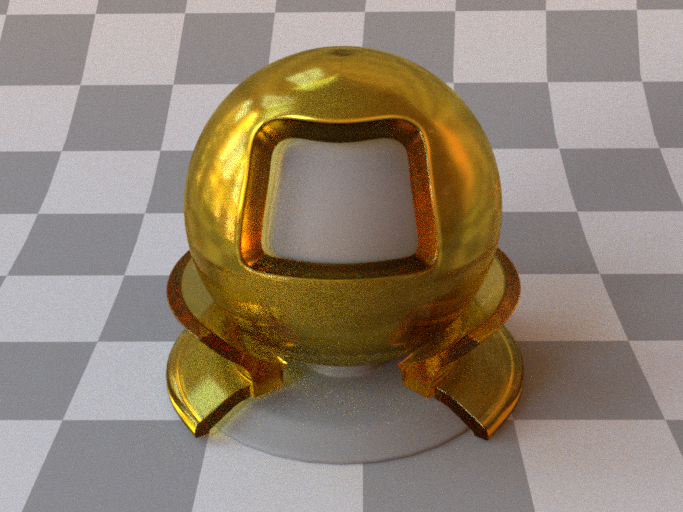
\includegraphics[width=0.5\linewidth]{imgs/disney_glass.png}
	\caption{Glass component of the Disney BSDF.}
\end{figure}

The 2012 version of the Disney BRDF did not support glasses. In the 2015 version, Burley added a dielectric lobe that is both transmissive and reflective using a standard microfacet-based refraction model~\cite{Walter:2007:MMR}:
\begin{equation}
f_{\text{glass}} = \begin{cases}
\frac{\text{baseColor} F_g D_g G_g}{4 |n \cdot \omega_{\text{in}}|} & \mbox{ if } \left(n_g \cdot \omega_{\text{in}}\right) \left(n_g \cdot \omega_{\text{out}}\right) > 0 \\
\frac{\sqrt{\text{baseColor}} (1 - F_g) D_g G_g \left|h \cdot \omega_{\text{out}} h \cdot \omega_{\text{in}} \right|}{
\left|n \cdot \omega_{\text{in}}\right| \left( h \cdot \omega_{\text{in}} + \eta h \cdot \omega_{\text{out}} \right)^2} & \mbox{ otherwise}\\
\end{cases}
\label{eq:f_glass}
\end{equation}

Note that for the refractive case (the second case), the color is taken square root for albedo preservation: a ray can refract twice inside an object.

For the Fresnel $F_g$, Burley found that the Schlick approximation was very inaccurate for $\eta \approx 1$ (up to $40 \times$ brighter than actual Fresnel), and decided to use the actual Fresnel equation for the dielectric materials. Unlike conductors, the Fresnel reflection for dielectric materials does not require complex indices of refraction and is much more intuitive to control. For completeness, the Fresnel equation is:
\begin{equation}
\begin{aligned}
F_g &= R_s^2 + R_p^2 \\
R_s &= \frac{h \cdot \omega_{\text{in}} - \eta h \cdot \omega_{\text{out}}}{h \cdot \omega_{\text{in}} + \eta h \cdot \omega_{\text{out}}} \\
R_p &= \frac{\eta h \cdot \omega_{\text{in}} - h \cdot \omega_{\text{out}}}{\eta h \cdot \omega_{\text{in}} + h \cdot \omega_{\text{out}}}
\end{aligned}
\end{equation}
again, note that we use the half-vector $h$ instead of the normal $n$, due to the microfacet assumption.

Sometimes we need to compute the Fresnel term solely using either the incoming direction or the outgoing direction. This can be done by using the Snell-Descartes law to convert $n \cdot \omega$ to the other one.

The normal distribution function $D_g$ and the masking-shadowing term $G_g$ are the same as the metal case.

\paragraph{Task (10\%).} You will implement the \lstinline{DisneyGlass} BRDF (Equation~\ref{eq:f_glass})
\begin{lstlisting}[language=c++]
// in material.h
struct DisneyGlass {
    Texture<Spectrum> base_color;
    Texture<Real> roughness;
    Texture<Real> anisotropic;

    Real eta; // internal IOR / externalIOR
};
\end{lstlisting}

You need to implement the following three functions in \lstinline{materials/disney_glass.inl}:
\begin{lstlisting}[language=c++]
Spectrum eval_op::operator()(const DisneyGlass &bsdf) const;
Real pdf_sample_bsdf_op::operator()(const DisneyGlass &bsdf) const;
std::optional<BSDFSampleRecord> sample_bsdf_op::operator()(const DisneyGlass &bsdf) const;
\end{lstlisting}

Lajolla already has an implementation of a dielectric glass in \lstinline{roughdielectric}. The only two differences are 1) the reflectance/transmittance color are handled differently and 2) the BSDF in \lstinline{roughdielectric} is isotropic. I suggest you start by copy-pasting or referencing the code from \lstinline{roughdielectric} and modify it.

Try out the scene \lstinline{scenes/disney_bsdf_test/disney_glass.xml} to see how the material look like. Play with the parameters.

\paragraph{Questions (5\%).} Answer these question(s) in a text file:
\begin{enumerate}
	\item Play with the index of refraction parameter $\eta$ (the physically plausible range is $[1, 2]$). How does it affect appearance?
	\item (Optional, not graded) Replace the dielectric Fresnel equation with a Schlick approximation (see Burley's course notes~\cite{Burley:2015:EDB} on the fix to the Schlick approximation to make it work for $\eta < 1$). Do you observe any differences when $\eta=1.5$? What about $\eta=1.01$?
\end{enumerate}

\section{Sheen}
\begin{figure}
	\centering
	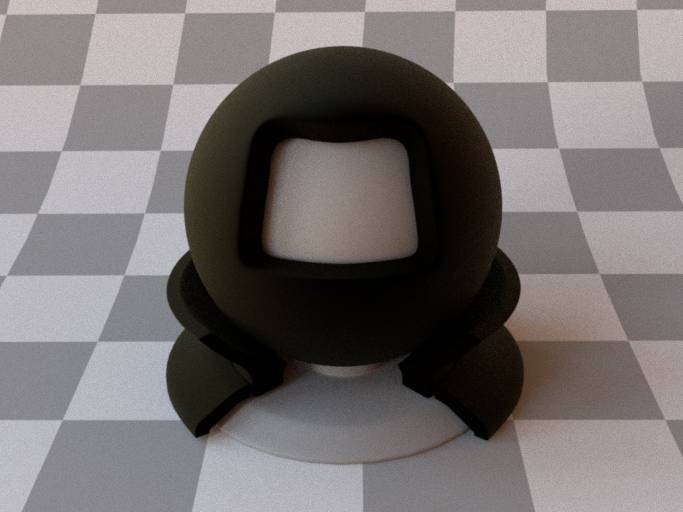
\includegraphics[width=0.5\linewidth]{imgs/disney_sheen.png}
	\caption{Sheen component of the Disney BSDF.}
\end{figure}

Materials such as clothes often exhibit strong responses at grazing angles. To compensate for this, Burley adds another component called the \emph{sheen} BRDF. Anything related to grazing angles can be done by hacking the Fresnel response (just like $f_{\text{diffuse}}$). The sheen BRDF is again a modified Schlick Fresnel:
\begin{equation}
\begin{aligned}
f_{\text{sheen}} &= C_{\text{sheen}} (1 - |h \cdot \omega_{\text{out}}|)^5 |n \cdot \omega_{\text{out}}| \\
C_{\text{sheen}} &= \left(1 - \text{sheenTint}\right) + \text{sheenTint} \cdot C_{\text{tint}} \\
C_{\text{tint}} &= \text{baseColor} / \text{luminance}(\text{baseColor}) \text{ if } \text{luminance}(\text{baseColor}) > 0 \text{ else } 1
\end{aligned}.
\label{eq:f_sheen}
\end{equation}

Here the color $C_{\text{sheen}}$ is a blending between the hue and saturation of the base color and white color based on the parameter $\text{sheenTint}$. Physical-wise, specular reflection caused by a dielectric material is usually achromatic when the index of refraction is the same across different wavelengths (and it often is). However, sheen is a BSDF for modeling strong retroreflection from clothes that are caused by the mesostructure of the cloth -- a much more complicated phenomonon. It is thus the best to give artists control here for how achromatic they want the retroreflection to be.

In the 2015 version of the Disney BSDF, the sheen component is applied for both the reflection and transmission. We only apply the sheen for the reflection here, since it is easier to sample and code.

\paragraph{Task (10\%).} You will implement the \lstinline{DisneySheen} BRDF (Equation~\ref{eq:f_sheen})
\begin{lstlisting}[language=c++]
// in material.h
struct DisneySheen {
    Texture<Spectrum> base_color;
    Texture<Real> sheen_tint;
};
\end{lstlisting}

You need to implement the following three functions in \lstinline{materials/disney_sheen.inl}:
\begin{lstlisting}[language=c++]
Spectrum eval_op::operator()(const DisneySheen &bsdf) const;
Real pdf_sample_bsdf_op::operator()(const DisneySheen &bsdf) const;
std::optional<BSDFSampleRecord> sample_bsdf_op::operator()(const DisneySheen &bsdf) const;
\end{lstlisting}

For sampling we will simply apply a cosine hemisphere sampling.

Try out \lstinline{scenes/disney_bsdf_test/simple_sphere.xml} and \lstinline{scenes/disney_bsdf_test/disney_sheen.xml} to see how the material look like. Play with the parameters.

\paragraph{Questions (5\%).} Answer these question(s) in a text file:
\begin{enumerate}
	\item Render the \lstinline{simple_sphere} scene with the sheen BRDF. What do you see? Why? What happens if you change the position of the light source?
\end{enumerate}

\section{Putting everything together}
Finally, we combine the five components we have and weigh them to get our final BSDF:
\begin{equation}
\begin{aligned}
f_{\text{disney}} =& (1 - \text{specularTransmission}) \cdot (1 - \text{metallic}) \cdot f_{\text{diffuse}} + \\
                   & (1 - \text{metallic}) \cdot f_{\text{sheen}} + \\
                   & (1 - \text{specularTransmission} \cdot (1 - \text{metallic})) \cdot \hat{f}_{\text{metal}} + \\
                   & 0.25 \cdot \text{clearcoat} \cdot f_{\text{clearcoat}} + \\
                   & (1 - \text{metallic}) \cdot \text{specularTransmission} \cdot f_{\text{glass}}
\end{aligned}
\label{eq:disney_bsdf}
\end{equation}

We need to modify the metal BRDF $\hat{f}_{\text{metal}}$ a bit: recall that our diffuse material is missing
a dielectric specular reflection. We include that in our metal BRDF. To do this, we modify the Fresnel term $F_m$ to include an achromatic specular component, with a control parameter $\text{specularTint}$ to potentially make it closer to the base color:
\begin{equation}
\begin{aligned}
	\hat{F}_m &= C_0 + (1 - C_0) (1 - \left(h \cdot n\right)^5) \\
	C_0 &= \text{specular} \cdot R_0(\eta) (1 - \text{metallic}) K_s + \text{metallic} \cdot \text{baseColor} \\
	K_s &= (1 - \text{specularTint}) + \text{specularTint} \cdot C_{\text{tint}}
\end{aligned}
\end{equation}

One complication when combining the glass BSDF and other BRDFs is that now we need to define the
behavior of the BRDF when the ray is \emph{inside} the object. The Disney BSDF technical notes do
not specify this. \href{https://github.com/mmp/pbrt-v3/issues/313}{Experiments} show that removing
all lobes except for the glass lobe when ray is inside the object (note that the glass still reflect
inside the object) gives more visually pleasing results. Therefore we define:
\begin{equation}
\begin{aligned}
	f_{\text{diffuse}} &= 0 \text{ if } \omega_{\text{in}} \cdot n_g \leq 0 \\
	f_{\text{metal}} &= 0 \text{ if } \omega_{\text{in}} \cdot n_g \leq 0 \\
	f_{\text{clearcoat}} &= 0 \text{ if } \omega_{\text{in}} \cdot n_g \leq 0 \\
	f_{\text{sheen}} &= 0 \text{ if } \omega_{\text{in}} \cdot n_g \leq 0
\end{aligned}.
\end{equation}

\paragraph{Task (20\%).} You will implement \lstinline{DisneyBSDF} (Equation~\ref{eq:disney_bsdf})
\begin{lstlisting}[language=c++]
// in material.h
struct DisneyBSDF {
    Texture<Spectrum> base_color;
    Texture<Real> specular_transmission;
    Texture<Real> metallic;
    Texture<Real> subsurface;
    Texture<Real> specular;
    Texture<Real> roughness;
    Texture<Real> specular_tint;
    Texture<Real> anisotropic;
    Texture<Real> sheen;
    Texture<Real> sheen_tint;
    Texture<Real> clearcoat;
    Texture<Real> clearcoat_gloss;

    Real eta;
};
\end{lstlisting}

You need to implement the following three functions in \lstinline{materials/disney_bsdf.inl}:
\begin{lstlisting}[language=c++]
Spectrum eval_op::operator()(const DisneyBSDF &bsdf) const;
Real pdf_sample_bsdf_op::operator()(const DisneyBSDF &bsdf) const;
std::optional<BSDFSampleRecord> sample_bsdf_op::operator()(const DisneyBSDF &bsdf) const;
\end{lstlisting}

For importance sampling, ignore the sheen component since it is relatively weak compared to other lobes. Randomly choose between a diffuse lobe, a metal lobe, a clearcoat lobe, and the glass lobes based on the following weights:
\begin{equation}
\begin{aligned}
\text{diffuseWeight} &= (1 - \text{metallic}) \cdot (1 - \text{specularTransmission}) \\
\text{metalWeight} &= (1 - \text{specularTransmission} \cdot (1 - \text{metallic})) \\
\text{glassWeight} &= (1 - \text{metallic}) \cdot \text{specularTransmission} \\
\text{clearcoatWeight} &= 0.25 \cdot \text{clearcoat}
\end{aligned}
\end{equation}
However, when the ray is from inside the object ($\omega_{\text{in}} \cdot n_g \leq 0$), we set all weights
to $0$ and only leave the glass lobes (note that glass still both reflect and refract).

When implementing, add one component at a time. Don't rush and put everything in there at once. Do sanity check with only enabling one component at a time. Note that even if everything other than the base color is set to zero, there is still a specular component from the dielectric specular response of the modified metal lobe. 

Also recall from homework 0: you might need to rescale your random number $w$ for selecting reflection/refraction.

Try out the scene \lstinline{scenes/disney_bsdf_test/disney_bsdf.xml} to see how the material look like. Play with the parameters.

\paragraph{Task (5\%).} Render an image that is not in the test scenes with your Disney BSDF! Play with textures and geometry to make it look interesting. Have fun!

\bibliographystyle{plain}
\bibliography{refs}

\end{document}